\section{Research Design And Methodology}\label{Methodology}

\subsection{Data}
We extracted raw data of M\&A deals  from the Thomson Reuters database. We decided to limit the data scope to certain remarks in terms of the wide extensive setting of the study to avoid incomplete dataset, i.e. to ensure data availability for each M\&A deal \cite{mackinlay1997}. 

Transactions covered M\&A deals between companies where target has been operating in software industry completed between 1981 and 2018 and acquired did not. We found 1551 deals where target companies were fulfilling the requirements and 10354 where acquiring companies met them. Next, one should have been limit the sample to leave only transaction resulting in change of control following the M\&A. The threshold describing change of control as buying exact \% of shares is different for each individual case and literature did not arrive to any plain conclusions in this matter (from 11\% (Almedia) to even 50\% in case of small private companies). Since no sensible guidelines can be found in the literature during collection process we limited the sample for deal above 5\% and later when performing econometric models we made a robustness checks and prepare models for different level of thresholds.

Since the research focuses on abnormal returns from the stock price we filtered the transactions where acquirer or target were publicly traded companies and so the stock prices were available. Table  \ref{table1}  present the breakdown and data selection statistics.

Should be recalled that there is a huge disproportion between data available for target companies and acquiring in favour of the second group. After considering, however, it seems to be reasonable. Acquirers typically are "the big ones" while targets are simply smaller entities. Since the stock exchange is dominated by the big companies no surprisingly in our database acquirers play the dominant role. To sum up our research consist of two data sets. First, are targets listed on stock exchange (1553 observations), second, are acquirers listed on stock exchange (10359 observations). Depending on the level of threshold when the change of control takes place (5\%, 11\% or 30\%) the available data for our research changes. All further results are presented for 5\% threshold but other levels were examined as well and delivered changeless results.

The target companies were from USA (24\%), Japan (14\%) and Canada (8\%). They were acquired by companies from financial (28\%), IT Consulting (10\%) and alternative financial investments sectors (8\%). All in all, financial sector was dominant as an acquirer taking over about 43,3\% of all targets in a data set. Its dominance, however, was observed only when examining the targets companies. With full


\small
\begin{center}

\begin{table}
  \caption{Summary statistics of database assuming 5\% change of control threshold}
  \label{table1}
  \begin{tabular}{p{1.5cm}p{1cm}p{1cm}p{1cm}p{1cm}p{1cm}p{1cm}}
\toprule
&& \textbf{Targets}& & &\textbf{Acquirers} & &
\midrule
& obs & mean & stdev & obs & mean & stdev\\
AR&859&0,055&0,154&7843&0,001&0,041\\
CAR3&859&0,115&0,243&7843&0,007&0,289\\
DealSize&636&328,2&1733,5&5279&91,425&262,9\\
NetIncome&582&-8,95&811.5&1161&34,6&213,6\\
acquired&859&40,0\%&37,5\%&10359&83,7\%&30,0\%\\
\midrule
\multicolumn{4}{l}{\textbf{Dummy variables:}}\\
domestic&859&76,4\%&&10359&72,1\%\\
finance&856&43,3\%&&10359&8,9\%\\
related&858&26,5\%&&10359&49,1\%\\
merger&859&23,2\%&&10359&23,1\%\\
TFA&859&29,2\%&&10359&18,6\%\\
AFA&859&30,5\%&&10359&14,7\%\\
friendly&859&84,5\%&&10359&94,4\%\\
bubble&859&5,59\%&&10359&19,6\%\\
\bottomrule
\end{tabular}
    \begin{tablenotes}
      \small
      \item TFA states for target financial advisor
      AFA states for acquirer financial advisor
      ARzero is abnormal return in the event day
      CAR3 is cumulative abnormal return in event window three days before and three days after announcement
    \end{tablenotes}
\end{table}

\end{center}



\subsection{Method} 

In order to verify hypothesis we have decided to conduct an event study that analyses the impact on a firm's stock values during public corporate M\&A announcements standardized by MacKinlay \cite{mackinlay1997} implemented by plenty of researchers so far (e.g. \cite{HENDRICKS2003501}, \cite{Fornell2006}).

We defined an event date as a public M\&A announcement. The estimation window consisted of 200 open trading days. The event window covered up to 10 day before and 10 days after announcement however other windows were analysed as well in order to ensure robustness of the results. We assumed market to be semi-strong efficient where the reaction time in the market is immediate and rapid but it might not always be the case that the effect of an event will only last for one day.  Furthermore, choosing a short event window mitigate the risk of getting the data affected by any interruptions (noise) from other corporate actions \cite{LegerYang2005}.

\begin{figure}[h]
  \centering
  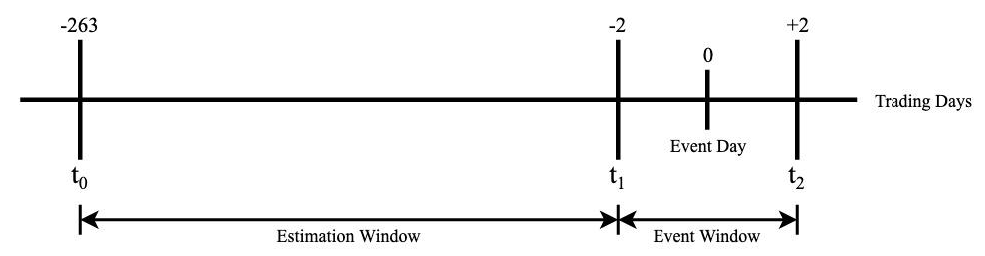
\includegraphics[width=\linewidth] {timline event.png}
  \caption{Time line of the event study}
  \label{Fig1}
\end{figure}


The objective with this event study is to analyze the abnormal returns around the M\&A announcement, i.e. the stock price deviation from the expected return in the pre-defined event window. Where the expected return for each firm was calculated/predicted, by using the ordinary least squares (OLS) to estimate the estimation window.  The normal return is defined as the return that would be expected if the event did not take place. In event studies, one has the privilege of following either a statistical model or an economic model when constructing a normal return model, in order to calculate abnormal returns. In other words, there is no significant benefits using an economic model over a statistical model \cite{mackinlay1997}. Consequently, a statistical model is the more ideal preference in this context.
There are two commonly known statistical models, the constant mean return model that is generally the most simple model of the two, where the normal return is defined as the average return (constant over time) in the estimation window or the market model  which is regarded as a potential improved version of the constant mean return model. Nevertheless, it was found \cite{BROWN1980205} that the results generated from the constant mean return model, and the market model are in fact very similar the market model is more universally used, and is also regarded as one of the most suitable estimation model for event studies. 

Thus, the market model was chosen for estimating the expected return on the stocks, and the Equation as follows \cite{mackinlay1997}:

\begin{equation}
AR = R_{it} - (\alpha_i + \beta_i * R_{mt})
\label{eqn:AR}
\end{equation}
where:\\
AR\_{it} = \text{abnormal return of a firm's stock i on day t} \\
R\_{it} = \text{actual return of a firm's stock i on day t} \\
\alpha\_i = \text{first regression parameter (y-intercept) of firm's stock i}  \\
\beta\_i = \text{second regression parameter (slope/regression coefficient) that  expresses the sensitivity of a firm's stock i to the market index m} \\
E(R\_{mt}) = \text{expected market return on day t}\\


If there is an intention of capturing the overall effect of the event over the event window, i.e. to estimate the total-firm stock movements during a new information and to test the abnormal returns. The cumulative abnormal return (CAR) needs to be calculated. Where CAR is simply the sum of the abnormal returns in the event windows.

\subsection{Measurement variables}

The dependent variable is represented by abnormal return. Consequently, the abnormal return can be used for quantifying an economic impact derived from an event, hence the economic impact reflects the variance of abnormal returns.

Based on the previous research that reported significant difference in abnormal returns for country effect and industry relatedness (see Section \ref{Sec2}), we used dummy variables describing domestic vs cross-border deals and related vs unrelated industry. As related industries we assumed to be (industry according to Thomson Database): computers and electronics, IT consulting, Telecommunications Services, E-commerce / B2B, Internet and Catalog Retailing, Computers \& Peripherals, Other High Technology and Other Telecom.

We used deal and firm related characteristics \cite{Cai2011} as control variables to account for other factors that may change the relationship between the dependent variable and independent variables.  Previous studies has shown promising conclusions finding that acquiring firms earn higher abnormal return if the \textbf{deal size} is large \cite{ALEXANDRIDIS2017}. This result is moderately contradicted by Fuller et al. \cite{fuller2002}, who find that larger target firms will require larger deal, which in turn will create negative impact on the abnormal return of the acquiring firm. This however was supported by Alexandridis et al. \cite{ALEXANDRIDIS20131}, who found that larger target firms generates lower abnormal return if the deal size is also large. Meanwhile, other studies found no significant relation between the abnormal return and the size of acquiring or target firm \cite{CAKICI1996307} .

Whether the transaction of a consolidation nature was so-called \textbf{hostile} takeover or not, is another potential determinant of the effects of consolidation processes. Many studies prove the occurrence of statistically significant positive rates of return due to hostile takeovers for the acquired companies' shareholders (\cite{Lounghran1997}, \cite{Rau1998}), however, in terms of the rates of return for shareholders of companies taking over such a division of transactions is no longer relevant (\cite{FRANKS1996163}, \cite{kini2004}). Among hostile takeovers, takeovers have only the highest returns, with only one hostile bidder \cite{sundersanam2006}.

Acquisitions made by over-valued companies (glamour), which were characterized by high \textbf{financial multiples}, were compared widely, as opposed to transactions of undervalued companies - those with low values of the described ratios. Rau and Vermaelen (1998) \cite{Rau1998} proved that acquisitions made by overvalued companies were characterized by higher rates of return during the transaction announcement period, while much lower during the 3 years after the transaction from other companies. In addition, they confirmed that such glamour transaction for the shareholders of the acquired company are more favorable than for the shareholders of the acquiring company. These results also supported other studies (\cite{sundersanam2003}, \cite{andrade}) giving the same results, however, on other samples. There is, however, inconsistent results in the literature, as a certain group of studies does not confirm the existence of such regularities \cite{mitchell2000}, \cite{dong2006}) and proves that there is no dependence of additional rates of return on whether the acquiring company is overvalued or neither The discrepancy of results is explained by the use of different methods of measuring the phenomenon of overvaluation. The reevaluation of companies is also associated with one of the theories saying that managers of overvalued companies are aware of this, so they protect the interests of shareholders against the fall in share prices that will occur after the bull market, trying to exchange overvalued shares for real acquired assets in the process of mergers and acquisitions (\cite{Gregory}, \cite{SHLEIFER2003295}). This phenomenon is classified by some researchers as issues related to the problem of information asymmetry (\cite{dierkens1991}). In database multiples were included calculating price to different financial position like net income, EBIT, EBITDA, sales or net asset.
Other characteristics that potentially might have had impact abnormal returns were: type of transaction - whether it was merger or acquisition, did target or acquire hire financial advisor, what percentage of shares was acquired and whether transaction took place in dotcom bubble. 

%\textbf{Test Procedure}

%Like many event studies, in order to determine whether if the abnormal returns within an event window are significant different from zero we used parametric and nonparametric tests.

%Given the fact that the market model is a linear regression and normality of the residuals (i.e. the difference between the observed value and the estimated value) is an assumption of a linear model, addresses the choice of using a parametric t-test to test the null hypothesis. A t-test is one of the most common tool within the field of event studies. That provides insight of whether if there is any significant difference (p < 0.05) between two sets of groups, by comparing the means. In other words, t-test determines if a null hypothesis is rejected or not. Which in turn signifies if the difference happened by chance or is reliable. That is, if the same outcome can be found in other assessments with the same data population. For example, in this case a t-test can detect the significance of the abnormal return caused by a M\&A announcement, where the null hypothesis and alternative hypothesis can be defined as following:
%• H0: AR = 0, the abnormal return is not significant different from the expected return (there is no relationship between the groups, i.e. the economic impact is not significant).
%• H1: AR ≠ 0, the abnormal return is significant different from the expected return (there is a relationship between the groups, i.e. the economic impact is significant).
%SOME MATH HERE 

%\textbf{Multiple Regression Analysis}
%3.6 Multiple Regression Analysis
%This thesis study has explored numerous potential independent variables that can explain the variance in the dependent variable. Thus, for the purpose of finding the best well establish relationship between the selected predictors and abnormal return during M\&A announcements, an ordinary least squares linear multiple regression analysis was conducted with the help of the statistical analysis program SPSS. By using a multiple regression analysis it is possible to include two or more independent variables at the same time. Which in turn can help in determine/finding the combination of significant predictors with the highest explanatory power of the variance in the abnormal return. Also, each significant predictor in this case, represents an economic impact on the abnormal return.
%Before commencing a multiple regression analysis, it is essential to create/collect a complete data set (at least as complete as possible). Depending on data availability the number of observation for a regression model will differ. Furthermore, some conditions needs to be met, in order for the data set to be acceptable. Such as, the variables in a regression model complies with the normality assumption (i.e. the residuals are normally distributed, which can be checked with a normal probability plot in SPSS), the independent variables are significant, and tested for correlation/multicollinearity (see more comprehensive description in respective sub-headers above). After the data set and the principle of the multiple regression model has been satisfied, a regression analysis can be carried out. Where the general interpretation of a significant variable in multiple regression analysis goes as following: for one unit increase in the explanatory/independent variable the model predicts that the dependent variable will increase or decrease (depending on the sign on the coefficient) by an amount units, holding all other explanatory/independent variables constant (fixed).
